\documentclass[11pt,a4paper]{article}

% --- Paquetes ---
\usepackage[utf8]{inputenc}
\usepackage[spanish,es-tabla,es-noquoting]{babel}
\usepackage[margin=2.5cm]{geometry}
\usepackage{amsmath,amssymb}
\usepackage{graphicx}
\usepackage{xcolor}
\usepackage{hyperref}
\usepackage{booktabs}
\usepackage{enumitem}
\usepackage{microtype}
\usepackage{titlesec}
\usepackage{fancyhdr}
\usepackage{tikz}
\usepackage{fontawesome5}
\usetikzlibrary{arrows.meta, positioning, shapes.geometric, calc}

% --- Configuración de hipervínculos ---
\hypersetup{
    colorlinks=true,
    linkcolor=blue!70!black,
    citecolor=blue!70!black,
    urlcolor=blue!70!black
}

% --- Encabezado y pie de página ---
\pagestyle{fancy}
\fancyhf{}
\lhead{\small Computación Paralela y Distribuida -- 2026-2}
\rhead{\small Tarea No. 03}
\cfoot{\thepage}

% --- Título e información ---
\title{\textbf{Universidad Nacional de Colombia}\\[0.3em]
\Large \textbf{Facultad de Ingeniería -- Departamento de Ingeniería de Sistemas e Industrial}\\[0.3em]
\large \textbf{Computación Paralela y Distribuida}\\
\large \textbf{Tarea No. 03: Ejercicios -- Paralelismo a Nivel de Tarea}}
\author{\textbf{Jonathan López}}
\date{}

\begin{document}

\maketitle

\vspace{1em}
\hrule
\vspace{1.5em}

% =========================================================================
% PUNTO 1
% =========================================================================
\section{¿Qué es un conjunto parcialmente ordenado (POSET)? Muestre cuáles serían las propiedades de un POSET con el conjunto de los divisores de un número entero.}
\subsection{¿Qué es un POSET?}
Un POSET es una estructura definida por $(S, \leq)$, donde $S$ es un conjunto con al menos un elemento y $\leq$ es una relación binaria que cumple las siguientes propiedades:
\begin{itemize}
    \item Reflexiva: $\forall a \in S,\; a \leq a$.
    \item Antisimétrica: $\forall a, b \in S,\; (a \leq b \wedge b \leq a) \implies a = b$.
    \item Transitiva: $\forall a, b, c \in S,\; (a \leq b \wedge b \leq c) \implies a \leq c$.
\end{itemize}
Cabe aclarar que, a diferencia de un conjunto totalmente ordenado, en un POSET pueden existir elementos $a, b \in S$ tales que no se cumple ni $a \leq b$ ni $b \leq a$. Se dice que estos elementos son incomparables y se denotan $a \parallel b$.

\subsection{POSET con el conjunto de divisores de un número entero}
Para $n \in \mathbb{Z}^+$, se define el POSET $D(n) = \{d \in \mathbb{Z}^+ : d \mid n \text{ ($d$ divide a $n$)}\}$, donde:
\[ a \mid b \iff \exists k \in \mathbb{Z}^+ \text{ tal que } b = k \cdot a \]
Las propiedades de este POSET son:
\begin{itemize}
    \item Reflexiva: $\forall a \in D(n),\; a \mid a$.
    \item Antisimétrica: $\forall a, b \in D(n),\; (a \mid b \wedge b \mid a) \implies a = b$.
    \item Transitiva: $\forall a, b, c \in D(n),\; (a \mid b \wedge b \mid c) \implies a \mid c$.
\end{itemize}

\subsection{Ejemplo de POSET con el conjunto de divisores de 24: $D(24)$}
Considerando $n = 24$, el conjunto de todos sus divisores positivos es:
\[ D(24) = \{1, 2, 3, 4, 6, 8, 12, 24\} \]

\noindent Las relaciones de cobertura ($a \lessdot b$, dependencias directas en el orden) corresponden a:
\[ \{1 \mid 2,\; 1 \mid 3,\; 2 \mid 4,\; 2 \mid 6,\; 3 \mid 6,\; 4 \mid 8,\; 4 \mid 12,\; 6 \mid 12,\; 8 \mid 24,\; 12 \mid 24\} \]

\noindent Los pares de \textbf{elementos incomparables} ($a \parallel b$, es decir, $a \nmid b$ y $b \nmid a$) corresponden a:
\[ \{2 \parallel 3,\; 3 \parallel 4,\; 3 \parallel 8,\; 4 \parallel 6,\; 6 \parallel 8,\; 8 \parallel 12\} \]

\begin{figure}[htbp]
\centering
\begin{tikzpicture}[
    hasse node/.style={circle, draw=blue!70!black, fill=blue!10, thick, minimum size=8mm, inner sep=0pt, font=\small\bfseries},
    hasse edge/.style={thick, draw=gray!70}
]
    % Nivel 0
    \node[hasse node] (n1) at (0, 0) {$1$};

    % Nivel 1
    \node[hasse node] (n2) at (-1.6, 1.4) {$2$};
    \node[hasse node] (n3) at (1.6, 1.4)  {$3$};

    % Nivel 2
    \node[hasse node] (n4) at (-1.6, 2.8) {$4$};
    \node[hasse node] (n6) at (1.6, 2.8)  {$6$};

    % Nivel 3
    \node[hasse node] (n8)  at (-1.6, 4.2) {$8$};
    \node[hasse node] (n12) at (1.6, 4.2)  {$12$};

    % Nivel 4
    \node[hasse node] (n24) at (0, 5.6) {$24$};

    % Aristas (Relaciones de cobertura)
    \draw[hasse edge] (n1) -- (n2);
    \draw[hasse edge] (n1) -- (n3);
    \draw[hasse edge] (n2) -- (n4);
    \draw[hasse edge] (n4) -- (n8);
    \draw[hasse edge] (n3) -- (n6);
    \draw[hasse edge] (n6) -- (n12);
    \draw[hasse edge] (n2) -- (n6);
    \draw[hasse edge] (n4) -- (n12);
    \draw[hasse edge] (n8) -- (n24);
    \draw[hasse edge] (n12) -- (n24);
\end{tikzpicture}
\caption{Diagrama de Hasse del POSET $(D(24), \mid)$.}
\label{fig:hasse_d24}
\end{figure}

\noindent En el diagrama de $D(24)$ podemos observar una correspondencia directa con un grafo computacional de tareas (DAG):
\begin{itemize}
    \item \textbf{Relaciones de orden (cadenas):} Modelan dependencias de precedencia entre tareas secuenciales (por ejemplo, para procesar la tarea $4$ se debe haber completado previamente la tarea $2$, y antes de esta, la tarea $1$).
    \item \textbf{Elementos incomparables (anticadenas):} Modelan tareas que no tienen dependencia mutua (como $4$ y $6$, o $8$ y $12$), por lo cual pueden ejecutarse de manera concurrente en procesadores independientes.
\end{itemize}
Por lo tanto, la estructura de un POSET proporciona el fundamento formal para modelar dependencias, sincronización y concurrencia en la ejecución de tareas en sistemas paralelos.

\vspace{2em}

% =========================================================================
% CONTEXTO Y FIGURA PARA PREGUNTAS 2 Y 3
% =========================================================================
\noindent Responda las preguntas 2 y 3 con base en la siguiente figura:

\begin{center}
    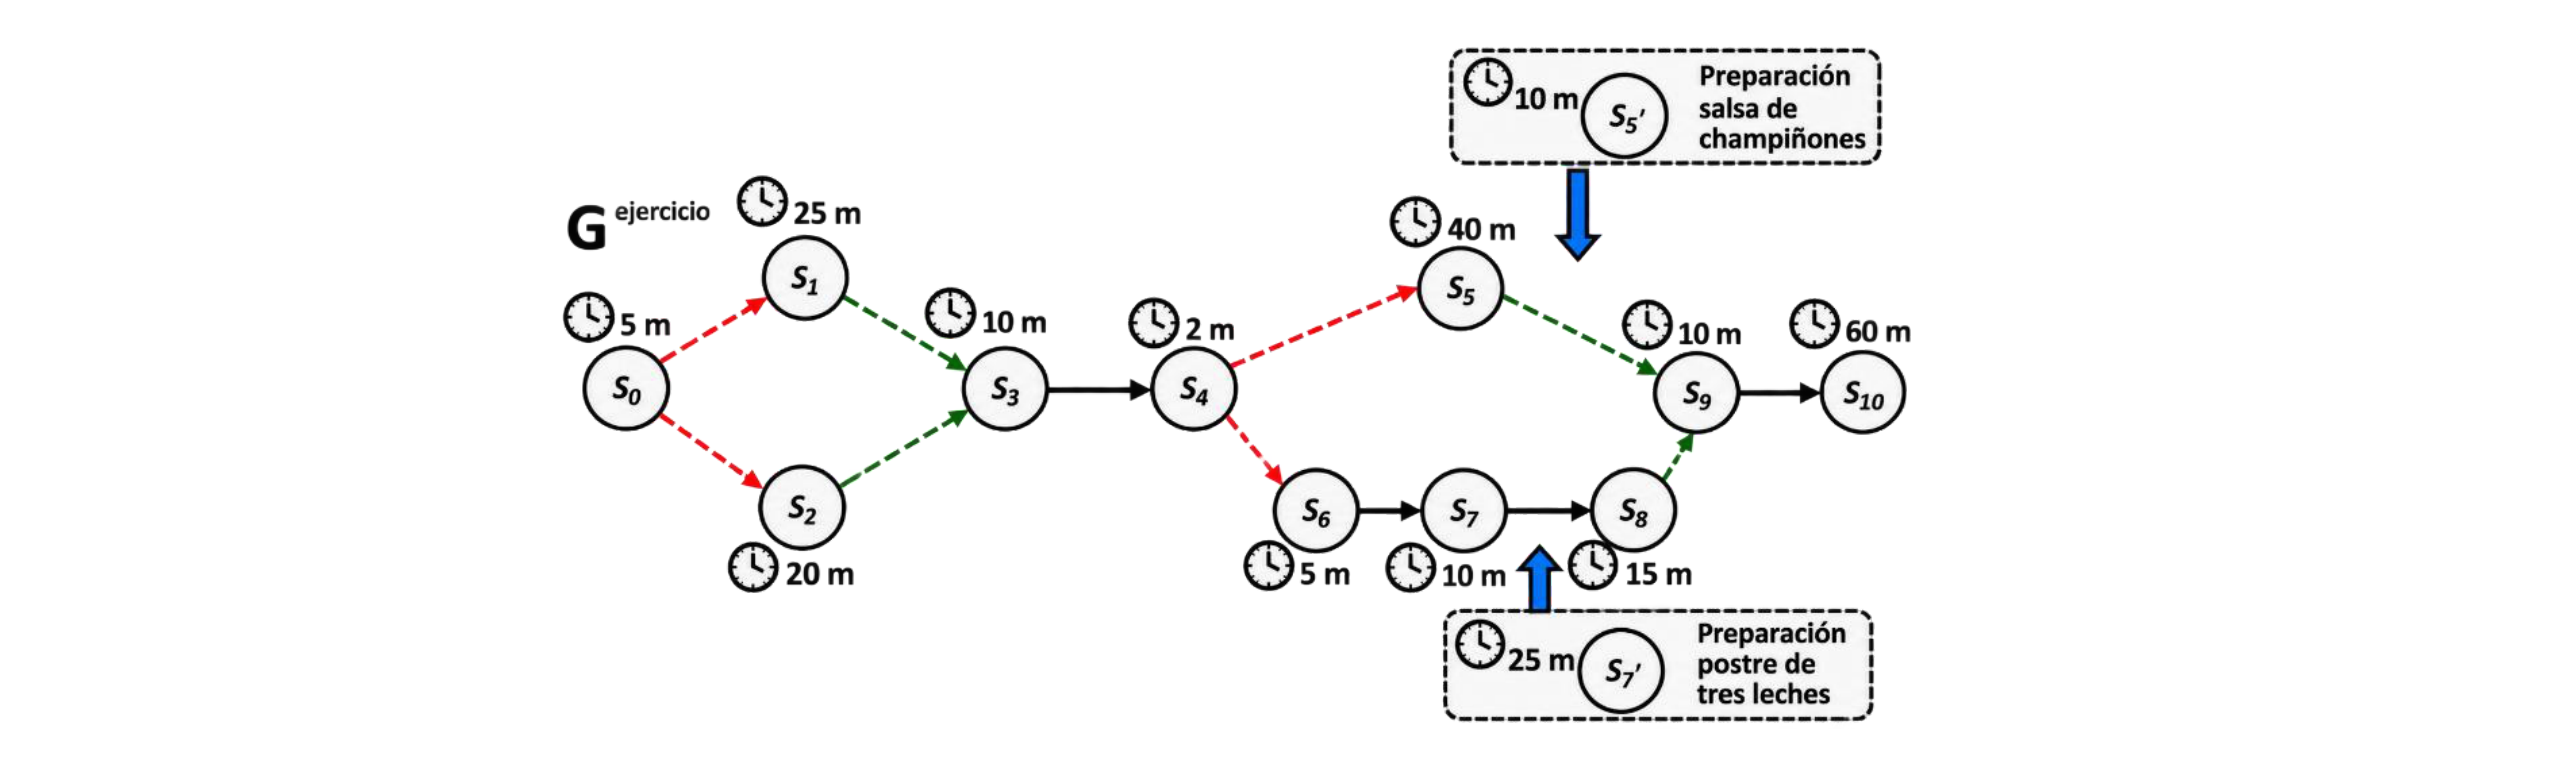
\includegraphics[width=\textwidth]{figura.png}
\end{center}

\vspace{1.5em}

% =========================================================================
% PUNTO 2
% =========================================================================
\section{Para el grafo computacional $G^{\text{ejercicio}}$ adicionarle las dos actividades indicadas en la ubicación que señalan las flechas azules en el diagrama. Después, calcule el $\text{WORK}(G^{\text{ejercicio}})$, el $\text{SPAN}(G^{\text{ejercicio}})$ y el paralelismo ideal correspondiente.}

\noindent\hspace*{-1cm}%
\begin{tikzpicture}[
    scale=0.85, every node/.append style={transform shape},
    % Definición de estilos
    state/.style={circle, draw, thick, minimum size=8mm, inner sep=1pt, font=\small},
    highlight/.style={circle, draw, thick, minimum size=8mm, inner sep=1pt, font=\small, fill=orange!30},
    time label/.style={font=\small\sffamily, text=black},
    red arrow/.style={->, >={Latex[length=2.5mm]}, dashed, red, thick},
    green arrow/.style={->, >={Latex[length=2.5mm]}, dashed, green!60!black, thick},
    black arrow/.style={->, >={Latex[length=2.5mm]}, thick}
]

    % --- NODOS PRINCIPALES ---
    \node[highlight, label={[time label]above left:\faClock\ 5 m}] (S0) {$S_0$};
    
    \node[highlight, above right=0.8cm and 1.5cm of S0, label={[time label]above:\faClock\ 25 m}] (S1) {$S_1$};
    \node[state, below right=0.8cm and 1.5cm of S0, label={[time label]below:\faClock\ 20 m}] (S2) {$S_2$};
    
    \node[highlight, below right=0.8cm and 1.5cm of S1, label={[time label]above:\faClock\ 10 m}] (S3) {$S_3$};
    \node[highlight, right=1.2cm of S3, label={[time label]above:\faClock\ 2 m}] (S4) {$S_4$};
    
    % Rama superior
    \node[state, above right=0.8cm and 1.5cm of S4, label={[time label]above:\faClock\ 40 m}] (S5) {$S_5$};
    \node[state, right=1.5cm of S5, label={[time label]above:\faClock\ 10 m}] (S5p) {$S_5'$};
    
    % Rama inferior (Resaltada)
    \node[highlight, below right=0.8cm and 1.5cm of S4, label={[time label]below:\faClock\ 5 m}] (S6) {$S_6$};
    \node[highlight, right=1cm of S6, label={[time label]below:\faClock\ 10 m}] (S7) {$S_7$};
    \node[highlight, right=1cm of S7, label={[time label]below:\faClock\ 25 m}] (S7p) {$S_7'$};
    \node[highlight, right=1cm of S7p, label={[time label]below:\faClock\ 15 m}] (S8) {$S_8$};
    
    % Nodos finales
    \node[highlight, above right=0.8cm and 1.5cm of S8, label={[time label]above:\faClock\ 10 m}] (S9) {$S_9$};
    \node[highlight, right=1.2cm of S9, label={[time label]above:\faClock\ 60 m}] (S10) {$S_{10}$};

    % Etiqueta del grafo
    \node[above left=0.5cm and 0cm of S1, font=\Large] {$\mathbf{G}^{\text{ejercicio2}}$};

    % --- CONEXIONES (ARISTAS) ---
    \draw[red arrow] (S0) -- (S1);
    \draw[red arrow] (S0) -- (S2);
    
    \draw[green arrow] (S1) -- (S3);
    \draw[green arrow] (S2) -- (S3);
    
    \draw[black arrow] (S3) -- (S4);
    
    % Conexiones rama superior
    \draw[red arrow] (S4) -- (S5);
    \draw[black arrow] (S5) -- (S5p);
    \draw[green arrow] (S5p) -- (S9);
    
    % Conexiones rama inferior
    \draw[red arrow] (S4) -- (S6);
    \draw[black arrow] (S6) -- (S7);
    \draw[black arrow] (S7) -- (S7p);
    \draw[black arrow] (S7p) -- (S8);
    
    \draw[green arrow] (S8) -- (S9);
    
    \draw[black arrow] (S9) -- (S10);

\end{tikzpicture}

El trabajo es la suma de todos los tiempos que tomaría ejecutar todas las tareas en un único procesador; por lo tanto, el $\text{WORK}$ es:
\[ \text{WORK}(G^{\text{ejercicio}}) = \sum_{i} T(S_i) = 5 + 25 + 20 + 10 + 2 + 40 + 10 + 5 + 10 + 25 + 15 + 10 + 60 = 237\text{ m} \]

El span es el camino secuencial más largo en el grafo (en este caso, el camino resaltado en naranja: $S_0 \to S_1 \to S_3 \to S_4 \to S_6 \to S_7 \to S_7' \to S_8 \to S_9 \to S_{10}$); por lo tanto, el $\text{SPAN}$ es:
\[ \text{SPAN}(G^{\text{ejercicio}}) = 5 + 25 + 10 + 2 + 5 + 10 + 25 + 15 + 10 + 60 = 167\text{ m} \]

Finalmente, el paralelismo ideal se define como $\text{WORK} / \text{SPAN}$; por lo tanto:
\[ \text{Paralelismo ideal} = \frac{\text{WORK}(G^{\text{ejercicio}})}{\text{SPAN}(G^{\text{ejercicio}})} = \frac{237}{167} \approx 1.42 \]
\vspace{2em}

% =========================================================================
% PUNTO 3
% =========================================================================
\section{Para el grafo computacional $G^{\text{ejercicio}}$, escribir el seudocódigo de inicio y terminación de tareas utilizando las ``palabras'' \texttt{async} y \texttt{finish}.}
En el modelo computacional estructurado con las primitivas \texttt{async} y \texttt{finish}:
\begin{itemize}[noitemsep]
    \item \texttt{async \{ Stmt \}}: Crea una tarea hija asíncrona que se ejecuta concurrentemente. El hilo invocador (\textbf{hilo padre}) continúa inmediatamente con la siguiente instrucción secuencial.
    \item \texttt{finish \{ Stmt \}}: Bloque de sincronización (\textit{join}). El hilo padre ejecuta las instrucciones dentro del bloque y suspende su salida hasta que todas las tareas asíncronas creadas dentro del ámbito de dicho \texttt{finish} hayan terminado.
\end{itemize}

\vspace{0.5em}
\noindent Para garantizar que el \textbf{hilo padre permanezca siempre ejecutando las actividades del camino crítico ($\text{SPAN}$)}:
\[ S_0 \to S_1 \to S_3 \to S_4 \to S_6 \to S_7 \to S_7' \to S_8 \to S_9 \to S_{10} \]
las tareas que se bifurcan por fuera de este camino crítico son las que se delegan al bloque \texttt{async}:
\begin{enumerate}[noitemsep]
    \item En la primera bifurcación, la actividad fuera del $\text{SPAN}$ es $S_2$ ($20\text{ m}$). Por ende, se despacha $S_2$ en un \texttt{async}, y el hilo padre continúa directamente con $S_1$ ($25\text{ m}$).
    \item En la segunda bifurcación, la rama fuera del $\text{SPAN}$ es la superior $S_5 \to S_5'$ ($40 + 10 = 50\text{ m}$ frente a $5 + 10 + 25 + 15 = 55\text{ m}$ de la rama inferior). Por ende, se despacha dicha rama en un \texttt{async}, mientras el hilo padre ejecuta secuencialmente $S_6 \to S_7 \to S_7' \to S_8$.
    \item En los nodos secuenciales ($S_0$, $S_3$, $S_4$, $S_9$, $S_{10}$), el hilo padre continúa su ejecución secuencial directa.
\end{enumerate}

\begin{verbatim}
S0(); // Hilo padre

finish {
    async {
        S2(); // Tarea concurrente
    }
    S1();     // El hilo padre continúa directamente por el SPAN
} // join: espera que termine S2 

S3(); // Hilo padre
S4(); // Hilo padre

finish {
    async {
        S5();
        S5_prime(); // Tareas concurrentes
    }
    // El hilo padre continúa ejecutando
    S6();
    S7();
    S7_prime();
    S8();
} // join: espera que termine la rama de S5 y S5'

S9();  // Hilo padre
S10(); // Hilo padre finaliza la ejecución
\end{verbatim}

\noindent \textbf{Nota:} Es igualmente válido y equivalente expresar ambas ramas explícitamente mediante \texttt{async} dentro del bloque \texttt{finish} (por ejemplo, \texttt{finish \{ async \{ S1(); \} async \{ S2(); \} \}}).\vspace{2em}


% =========================================================================
% PUNTO 4
% =========================================================================
\section{El siguiente seudo-código, suma dos matrices triangulares inferiores (matrices cuadradas $n \times n$ en las cuales los elementos por encima de la diagonal, incluyendo la diagonal de $(0,0)$ a $(n,n)$, son cero). En el código, cada ejecución de la sentencia \texttt{A[i][j] = B[i][j] + C[i][j];} representa una unidad de tiempo en el grafo computacional correspondiente.}

\begin{verbatim}
finish {
    for (int i = 0; i < n; i++) { 
        async {
            for (int j = 0; j < i; j++) { 
                A[i][j] = B[i][j] + C[i][j];
            } // for-j
        } // async
    } // for-i
} // finish
\end{verbatim}

\vspace{0.8em}
\noindent En términos de $n$ ¿Cuál es el WORK del código mostrado? Explique cómo obtuvo su respuesta.

Iniciamos analizando de adentro hacia afuera: el bucle interno \texttt{for (int j = 0; j < i; j++)} ejecuta exactamente $i$ iteraciones, donde cada iteración equivale a una unidad de tiempo. A su vez, el bucle externo \texttt{for (int i = 0; i < n; i++)} realiza exactamente $n$ iteraciones (desde $i = 0$ hasta $i = n-1$). En cada una de estas iteraciones, el bucle interno representa $i$ unidades de tiempo. Así, la primera iteración del bucle externo ($i=0$) toma 0 unidades, la segunda ($i=1$) 1 unidad, la tercera 2 unidades, y así sucesivamente hasta la última iteración ($i=n-1$) que toma $n-1$ unidades de tiempo. Por lo tanto, el $\text{WORK}$ total es la suma de todas estas unidades de tiempo:
\[ \text{WORK} = 0 + 1 + 2 + \dots + (n-1) = \sum_{i=0}^{n-1} i = \frac{(n-1)n}{2} = \frac{n^2 - n}{2} \]
Así, el $\text{WORK}$ del código mostrado es $\frac{n^2 - n}{2}$ unidades de tiempo.


\end{document}
